\documentclass[1p]{elsarticle_modified}
%\bibliographystyle{elsarticle-num}

%\usepackage[colorlinks]{hyperref}
%\usepackage{abbrmath_seonhwa} %\Abb, \Ascr, \Acal ,\Abf, \Afrak
\usepackage{amsfonts}
\usepackage{amssymb}
\usepackage{amsmath}
\usepackage{amsthm}
\usepackage{scalefnt}
\usepackage{amsbsy}
\usepackage{kotex}
\usepackage{caption}
\usepackage{subfig}
\usepackage{color}
\usepackage{graphicx}
\usepackage{xcolor} %% white, black, red, green, blue, cyan, magenta, yellow
\usepackage{float}
\usepackage{setspace}
\usepackage{hyperref}

\usepackage{tikz}
\usetikzlibrary{arrows}

\usepackage{multirow}
\usepackage{array} % fixed length table
\usepackage{hhline}

%%%%%%%%%%%%%%%%%%%%%
\makeatletter
\renewcommand*\env@matrix[1][\arraystretch]{%
	\edef\arraystretch{#1}%
	\hskip -\arraycolsep
	\let\@ifnextchar\new@ifnextchar
	\array{*\c@MaxMatrixCols c}}
\makeatother %https://tex.stackexchange.com/questions/14071/how-can-i-increase-the-line-spacing-in-a-matrix
%%%%%%%%%%%%%%%

\usepackage[normalem]{ulem}

\newcommand{\msout}[1]{\ifmmode\text{\sout{\ensuremath{#1}}}\else\sout{#1}\fi}
%SOURCE: \msout is \stkout macro in https://tex.stackexchange.com/questions/20609/strikeout-in-math-mode

\newcommand{\cancel}[1]{
	\ifmmode
	{\color{red}\msout{#1}}
	\else
	{\color{red}\sout{#1}}
	\fi
}

\newcommand{\add}[1]{
	{\color{blue}\uwave{#1}}
}

\newcommand{\replace}[2]{
	\ifmmode
	{\color{red}\msout{#1}}{\color{blue}\uwave{#2}}
	\else
	{\color{red}\sout{#1}}{\color{blue}\uwave{#2}}
	\fi
}

\newcommand{\Sol}{\mathcal{S}} %segment
\newcommand{\D}{D} %diagram
\newcommand{\A}{\mathcal{A}} %arc


%%%%%%%%%%%%%%%%%%%%%%%%%%%%%5 test

\def\sl{\operatorname{\textup{SL}}(2,\Cbb)}
\def\psl{\operatorname{\textup{PSL}}(2,\Cbb)}
\def\quan{\mkern 1mu \triangleright \mkern 1mu}

\theoremstyle{definition}
\newtheorem{thm}{Theorem}[section]
\newtheorem{prop}[thm]{Proposition}
\newtheorem{lem}[thm]{Lemma}
\newtheorem{ques}[thm]{Question}
\newtheorem{cor}[thm]{Corollary}
\newtheorem{defn}[thm]{Definition}
\newtheorem{exam}[thm]{Example}
\newtheorem{rmk}[thm]{Remark}
\newtheorem{alg}[thm]{Algorithm}

\newcommand{\I}{\sqrt{-1}}
\begin{document}

%\begin{frontmatter}
%
%\title{Boundary parabolic representations of knots up to 8 crossings}
%
%%% Group authors per affiliation:
%\author{Yunhi Cho} 
%\address{Department of Mathematics, University of Seoul, Seoul, Korea}
%\ead{yhcho@uos.ac.kr}
%
%
%\author{Seonhwa Kim} %\fnref{s_kim}}
%\address{Center for Geometry and Physics, Institute for Basic Science, Pohang, 37673, Korea}
%\ead{ryeona17@ibs.re.kr}
%
%\author{Hyuk Kim}
%\address{Department of Mathematical Sciences, Seoul National University, Seoul 08826, Korea}
%\ead{hyukkim@snu.ac.kr}
%
%\author{Seokbeom Yoon}
%\address{Department of Mathematical Sciences, Seoul National University, Seoul, 08826,  Korea}
%\ead{sbyoon15@snu.ac.kr}
%
%\begin{abstract}
%We find all boundary parabolic representation of knots up to 8 crossings.
%
%\end{abstract}
%\begin{keyword}
%    \MSC[2010] 57M25 
%\end{keyword}
%
%\end{frontmatter}

%\linenumbers
%\tableofcontents
%
\newcommand\colored[1]{\textcolor{white}{\rule[-0.35ex]{0.8em}{1.4ex}}\kern-0.8em\color{red} #1}%
%\newcommand\colored[1]{\textcolor{white}{ #1}\kern-2.17ex	\textcolor{white}{ #1}\kern-1.81ex	\textcolor{white}{ #1}\kern-2.15ex\color{red}#1	}

{\Large $\underline{12n_{0092}~(K12n_{0092})}$}

\setlength{\tabcolsep}{10pt}
\renewcommand{\arraystretch}{1.6}
\vspace{1cm}\begin{tabular}{m{100pt}>{\centering\arraybackslash}m{274pt}}
\multirow{5}{120pt}{
	\centering
	\includegraphics[width=112pt]{../../../GIT/diagram.site/Diagrams/png/2181_12n_0092.png}\\
\ \ \ A knot diagram\footnotemark}&
\allowdisplaybreaks
\textbf{Linearized knot diagam} \\
\cline{2-2}
 &
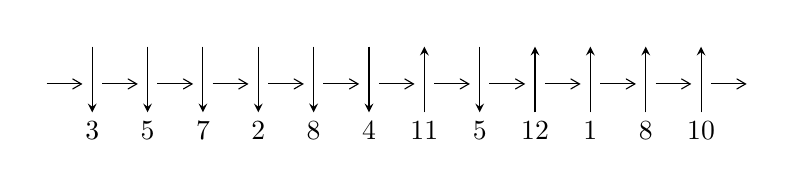
\begin{tikzpicture}[x=20pt, y=17pt]
	% nodes
	\node (C0) at (0, 0) {};
	\node (C1) at (1, 0) {};
	\node (C1U) at (1, +1) {};
	\node (C1D) at (1, -1) {3};

	\node (C2) at (2, 0) {};
	\node (C2U) at (2, +1) {};
	\node (C2D) at (2, -1) {5};

	\node (C3) at (3, 0) {};
	\node (C3U) at (3, +1) {};
	\node (C3D) at (3, -1) {7};

	\node (C4) at (4, 0) {};
	\node (C4U) at (4, +1) {};
	\node (C4D) at (4, -1) {2};

	\node (C5) at (5, 0) {};
	\node (C5U) at (5, +1) {};
	\node (C5D) at (5, -1) {8};

	\node (C6) at (6, 0) {};
	\node (C6U) at (6, +1) {};
	\node (C6D) at (6, -1) {4};

	\node (C7) at (7, 0) {};
	\node (C7U) at (7, +1) {};
	\node (C7D) at (7, -1) {11};

	\node (C8) at (8, 0) {};
	\node (C8U) at (8, +1) {};
	\node (C8D) at (8, -1) {5};

	\node (C9) at (9, 0) {};
	\node (C9U) at (9, +1) {};
	\node (C9D) at (9, -1) {12};

	\node (C10) at (10, 0) {};
	\node (C10U) at (10, +1) {};
	\node (C10D) at (10, -1) {1};

	\node (C11) at (11, 0) {};
	\node (C11U) at (11, +1) {};
	\node (C11D) at (11, -1) {8};

	\node (C12) at (12, 0) {};
	\node (C12U) at (12, +1) {};
	\node (C12D) at (12, -1) {10};
	\node (C13) at (13, 0) {};

	% arrows
	\draw[->,>={angle 60}]
	(C0) edge (C1) (C1) edge (C2) (C2) edge (C3) (C3) edge (C4) (C4) edge (C5) (C5) edge (C6) (C6) edge (C7) (C7) edge (C8) (C8) edge (C9) (C9) edge (C10) (C10) edge (C11) (C11) edge (C12) (C12) edge (C13) ;	\draw[->,>=stealth]
	(C1U) edge (C1D) (C2U) edge (C2D) (C3U) edge (C3D) (C4U) edge (C4D) (C5U) edge (C5D) (C6U) edge (C6D) (C7D) edge (C7U) (C8U) edge (C8D) (C9D) edge (C9U) (C10D) edge (C10U) (C11D) edge (C11U) (C12D) edge (C12U) ;
	\end{tikzpicture} \\
\hhline{~~} \\& 
\textbf{Solving Sequence} \\ \cline{2-2} 
 &
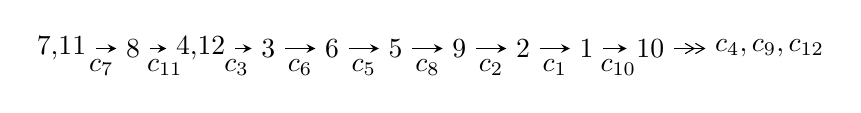
\begin{tikzpicture}[x=23pt, y=7pt]
	% node
	\node (A0) at (-1/8, 0) {7,11};
	\node (A1) at (1, 0) {8};
	\node (A2) at (33/16, 0) {4,12};
	\node (A3) at (25/8, 0) {3};
	\node (A4) at (33/8, 0) {6};
	\node (A5) at (41/8, 0) {5};
	\node (A6) at (49/8, 0) {9};
	\node (A7) at (57/8, 0) {2};
	\node (A8) at (65/8, 0) {1};
	\node (A9) at (73/8, 0) {10};
	\node (C1) at (1/2, -1) {$c_{7}$};
	\node (C2) at (3/2, -1) {$c_{11}$};
	\node (C3) at (21/8, -1) {$c_{3}$};
	\node (C4) at (29/8, -1) {$c_{6}$};
	\node (C5) at (37/8, -1) {$c_{5}$};
	\node (C6) at (45/8, -1) {$c_{8}$};
	\node (C7) at (53/8, -1) {$c_{2}$};
	\node (C8) at (61/8, -1) {$c_{1}$};
	\node (C9) at (69/8, -1) {$c_{10}$};
	\node (A10) at (11, 0) {$c_{4},c_{9},c_{12}$};

	% edge
	\draw[->,>=stealth]	
	(A0) edge (A1) (A1) edge (A2) (A2) edge (A3) (A3) edge (A4) (A4) edge (A5) (A5) edge (A6) (A6) edge (A7) (A7) edge (A8) (A8) edge (A9) ;
	\draw[->>,>={angle 60}]	
	(A9) edge (A10);
\end{tikzpicture} \\ 

\end{tabular} \\

\footnotetext{
The image of knot diagram is generated by the software ``\textbf{Draw programme}" developed by Andrew Bartholomew(\url{http://www.layer8.co.uk/maths/draw/index.htm\#Running-draw}), where we modified some parts for our purpose(\url{https://github.com/CATsTAILs/LinksPainter}).
}\phantom \\ \newline 
\centering \textbf{Ideals for irreducible components\footnotemark of $X_{\text{par}}$} 
 
\begin{align*}
I^u_{1}&=\langle 
-2.63090\times10^{169} u^{64}-1.19407\times10^{170} u^{63}+\cdots+5.11342\times10^{169} b-2.60080\times10^{170},\\
\phantom{I^u_{1}}&\phantom{= \langle  }-1.33678\times10^{170} u^{64}-5.86621\times10^{170} u^{63}+\cdots+1.27836\times10^{169} a-8.83930\times10^{170},\\
\phantom{I^u_{1}}&\phantom{= \langle  }u^{65}+5 u^{64}+\cdots+4 u+4\rangle \\
I^u_{2}&=\langle 
13 a^2 u+10 a^2+22 a u+61 b+31 a+11 u+46,\;a^3+a^2 u-7 a u+13 a- u+4,\;u^2- u-1\rangle \\
I^u_{3}&=\langle 
b,\;5 u^2+a+2 u+9,\;u^3+u^2+2 u+1\rangle \\
\\
I^v_{1}&=\langle 
a,\;3 b+v-5,\;v^2-7 v+1\rangle \\
\end{align*}
\raggedright * 4 irreducible components of $\dim_{\mathbb{C}}=0$, with total 76 representations.\\
\footnotetext{All coefficients of polynomials are rational numbers. But the coefficients are sometimes approximated in decimal forms when there is not enough margin.}
\newpage
\renewcommand{\arraystretch}{1}
\centering \section*{I. $I^u_{1}= \langle -2.63\times10^{169} u^{64}-1.19\times10^{170} u^{63}+\cdots+5.11\times10^{169} b-2.60\times10^{170},\;-1.34\times10^{170} u^{64}-5.87\times10^{170} u^{63}+\cdots+1.28\times10^{169} a-8.84\times10^{170},\;u^{65}+5 u^{64}+\cdots+4 u+4 \rangle$}
\flushleft \textbf{(i) Arc colorings}\\
\begin{tabular}{m{7pt} m{180pt} m{7pt} m{180pt} }
\flushright $a_{7}=$&$\begin{pmatrix}1\\0\end{pmatrix}$ \\
\flushright $a_{11}=$&$\begin{pmatrix}0\\u\end{pmatrix}$ \\
\flushright $a_{8}=$&$\begin{pmatrix}1\\- u^2\end{pmatrix}$ \\
\flushright $a_{4}=$&$\begin{pmatrix}10.4570 u^{64}+45.8887 u^{63}+\cdots-20.3543 u+69.1458\\0.514509 u^{64}+2.33517 u^{63}+\cdots-12.7222 u+5.08623\end{pmatrix}$ \\
\flushright $a_{12}=$&$\begin{pmatrix}u\\- u^3+u\end{pmatrix}$ \\
\flushright $a_{3}=$&$\begin{pmatrix}10.9715 u^{64}+48.2239 u^{63}+\cdots-33.0765 u+74.2321\\0.514509 u^{64}+2.33517 u^{63}+\cdots-12.7222 u+5.08623\end{pmatrix}$ \\
\flushright $a_{6}=$&$\begin{pmatrix}-2.56076 u^{64}-11.3025 u^{63}+\cdots+22.7562 u-15.2103\\-0.519422 u^{64}-2.45761 u^{63}+\cdots+16.9006 u-7.52354\end{pmatrix}$ \\
\flushright $a_{5}=$&$\begin{pmatrix}-3.92828 u^{64}-17.5296 u^{63}+\cdots+43.8945 u-28.7392\\-0.226329 u^{64}-1.14246 u^{63}+\cdots+13.8722 u-5.08179\end{pmatrix}$ \\
\flushright $a_{9}=$&$\begin{pmatrix}-0.467988 u^{64}-1.95761 u^{63}+\cdots-13.3003 u+0.571683\\1.21392 u^{64}+5.72728 u^{63}+\cdots-42.4563 u+17.1644\end{pmatrix}$ \\
\flushright $a_{2}=$&$\begin{pmatrix}11.9804 u^{64}+52.6553 u^{63}+\cdots-42.2932 u+79.5227\\-0.226329 u^{64}-1.14246 u^{63}+\cdots+13.8722 u-5.08179\end{pmatrix}$ \\
\flushright $a_{1}=$&$\begin{pmatrix}-1.45833 u^{64}-6.68429 u^{63}+\cdots+28.8135 u-15.0633\\-0.990343 u^{64}-4.72668 u^{63}+\cdots+42.1137 u-15.6350\end{pmatrix}$ \\
\flushright $a_{10}=$&$\begin{pmatrix}-0.205715 u^{64}-0.764176 u^{63}+\cdots-16.7041 u+3.00115\\1.42293 u^{64}+6.67656 u^{63}+\cdots-45.2828 u+19.1221\end{pmatrix}$\\&\end{tabular}
\flushleft \textbf{(ii) Obstruction class $= -1$}\\~\\
\flushleft \textbf{(iii) Cusp Shapes $= -250.136 u^{64}-1099.53 u^{63}+\cdots+889.233 u-1633.12$}\\~\\
\newpage\renewcommand{\arraystretch}{1}
\flushleft \textbf{(iv) u-Polynomials at the component}\newline \\
\begin{tabular}{m{50pt}|m{274pt}}
Crossings & \hspace{64pt}u-Polynomials at each crossing \\
\hline $$\begin{aligned}c_{1}\end{aligned}$$&$\begin{aligned}
&u^{65}+35 u^{64}+\cdots+4379 u+1
\end{aligned}$\\
\hline $$\begin{aligned}c_{2},c_{4}\end{aligned}$$&$\begin{aligned}
&u^{65}-7 u^{64}+\cdots-61 u-1
\end{aligned}$\\
\hline $$\begin{aligned}c_{3},c_{6}\end{aligned}$$&$\begin{aligned}
&u^{65}-4 u^{64}+\cdots-4 u-8
\end{aligned}$\\
\hline $$\begin{aligned}c_{5},c_{8}\end{aligned}$$&$\begin{aligned}
&u^{65}-3 u^{64}+\cdots+224 u-64
\end{aligned}$\\
\hline $$\begin{aligned}c_{7},c_{11}\end{aligned}$$&$\begin{aligned}
&u^{65}-5 u^{64}+\cdots+4 u-4
\end{aligned}$\\
\hline $$\begin{aligned}c_{9},c_{10},c_{12}\end{aligned}$$&$\begin{aligned}
&u^{65}+7 u^{64}+\cdots+88 u-1
\end{aligned}$\\
\hline
\end{tabular}\\~\\
\newpage\renewcommand{\arraystretch}{1}
\flushleft \textbf{(v) Riley Polynomials at the component}\newline \\
\begin{tabular}{m{50pt}|m{274pt}}
Crossings & \hspace{64pt}Riley Polynomials at each crossing \\
\hline $$\begin{aligned}c_{1}\end{aligned}$$&$\begin{aligned}
&y^{65}-3 y^{64}+\cdots+19078099 y-1
\end{aligned}$\\
\hline $$\begin{aligned}c_{2},c_{4}\end{aligned}$$&$\begin{aligned}
&y^{65}-35 y^{64}+\cdots+4379 y-1
\end{aligned}$\\
\hline $$\begin{aligned}c_{3},c_{6}\end{aligned}$$&$\begin{aligned}
&y^{65}+24 y^{64}+\cdots+7056 y-64
\end{aligned}$\\
\hline $$\begin{aligned}c_{5},c_{8}\end{aligned}$$&$\begin{aligned}
&y^{65}-47 y^{64}+\cdots+283648 y-4096
\end{aligned}$\\
\hline $$\begin{aligned}c_{7},c_{11}\end{aligned}$$&$\begin{aligned}
&y^{65}-21 y^{64}+\cdots+1448 y-16
\end{aligned}$\\
\hline $$\begin{aligned}c_{9},c_{10},c_{12}\end{aligned}$$&$\begin{aligned}
&y^{65}-55 y^{64}+\cdots+6134 y-1
\end{aligned}$\\
\hline
\end{tabular}\\~\\
\newpage\flushleft \textbf{(vi) Complex Volumes and Cusp Shapes}
$$\begin{array}{c|c|c}  
\text{Solutions to }I^u_{1}& \I (\text{vol} + \sqrt{-1}CS) & \text{Cusp shape}\\
 \hline 
\begin{aligned}
u &= -0.852107 + 0.536554 I \\
a &= \phantom{-}0.312816 - 0.088889 I \\
b &= -1.40349 + 0.30161 I\end{aligned}
 & \phantom{-}1.38895 - 2.95818 I & \phantom{-0.000000 } 0 \\ \hline\begin{aligned}
u &= -0.852107 - 0.536554 I \\
a &= \phantom{-}0.312816 + 0.088889 I \\
b &= -1.40349 - 0.30161 I\end{aligned}
 & \phantom{-}1.38895 + 2.95818 I & \phantom{-0.000000 } 0 \\ \hline\begin{aligned}
u &= -0.948009 + 0.367228 I \\
a &= \phantom{-}0.850963 - 0.753331 I \\
b &= \phantom{-}0.153663 + 0.857675 I\end{aligned}
 & \phantom{-}2.10912 - 0.34030 I & \phantom{-0.000000 } 0 \\ \hline\begin{aligned}
u &= -0.948009 - 0.367228 I \\
a &= \phantom{-}0.850963 + 0.753331 I \\
b &= \phantom{-}0.153663 - 0.857675 I\end{aligned}
 & \phantom{-}2.10912 + 0.34030 I & \phantom{-0.000000 } 0 \\ \hline\begin{aligned}
u &= -1.024770 + 0.135153 I \\
a &= -0.04125 + 1.56220 I \\
b &= -0.13124 - 1.75548 I\end{aligned}
 & \phantom{-}9.17254 - 3.64107 I & \phantom{-0.000000 } 0 \\ \hline\begin{aligned}
u &= -1.024770 - 0.135153 I \\
a &= -0.04125 - 1.56220 I \\
b &= -0.13124 + 1.75548 I\end{aligned}
 & \phantom{-}9.17254 + 3.64107 I & \phantom{-0.000000 } 0 \\ \hline\begin{aligned}
u &= -0.691259 + 0.784338 I \\
a &= -0.662548 + 0.346420 I \\
b &= -0.470514 - 0.941528 I\end{aligned}
 & \phantom{-}0.56978 - 4.38703 I & \phantom{-0.000000 } 0 \\ \hline\begin{aligned}
u &= -0.691259 - 0.784338 I \\
a &= -0.662548 - 0.346420 I \\
b &= -0.470514 + 0.941528 I\end{aligned}
 & \phantom{-}0.56978 + 4.38703 I & \phantom{-0.000000 } 0 \\ \hline\begin{aligned}
u &= \phantom{-}0.916883 + 0.120007 I \\
a &= -0.389774 + 0.653279 I \\
b &= -0.947907 - 0.877633 I\end{aligned}
 & \phantom{-}3.47356 + 1.55230 I & \phantom{-0.000000 } 0 \\ \hline\begin{aligned}
u &= \phantom{-}0.916883 - 0.120007 I \\
a &= -0.389774 - 0.653279 I \\
b &= -0.947907 + 0.877633 I\end{aligned}
 & \phantom{-}3.47356 - 1.55230 I & \phantom{-0.000000 } 0\\
 \hline 
 \end{array}$$\newpage$$\begin{array}{c|c|c}  
\text{Solutions to }I^u_{1}& \I (\text{vol} + \sqrt{-1}CS) & \text{Cusp shape}\\
 \hline 
\begin{aligned}
u &= \phantom{-}0.568857 + 0.725937 I \\
a &= \phantom{-}0.442387 + 0.229414 I \\
b &= -0.895487 - 0.532333 I\end{aligned}
 & -2.18618 - 0.21906 I & \phantom{-0.000000 } 0 \\ \hline\begin{aligned}
u &= \phantom{-}0.568857 - 0.725937 I \\
a &= \phantom{-}0.442387 - 0.229414 I \\
b &= -0.895487 + 0.532333 I\end{aligned}
 & -2.18618 + 0.21906 I & \phantom{-0.000000 } 0 \\ \hline\begin{aligned}
u &= -0.842958 + 0.701034 I \\
a &= -0.402908 + 1.148860 I \\
b &= \phantom{-}0.613031 - 0.666960 I\end{aligned}
 & -1.58736 + 0.20570 I & \phantom{-0.000000 } 0 \\ \hline\begin{aligned}
u &= -0.842958 - 0.701034 I \\
a &= -0.402908 - 1.148860 I \\
b &= \phantom{-}0.613031 + 0.666960 I\end{aligned}
 & -1.58736 - 0.20570 I & \phantom{-0.000000 } 0 \\ \hline\begin{aligned}
u &= \phantom{-}0.322386 + 0.842732 I \\
a &= -0.573249 + 1.009110 I \\
b &= \phantom{-}0.004484 + 1.102400 I\end{aligned}
 & \phantom{-}4.65051 + 1.43055 I & \phantom{-0.000000 } 0 \\ \hline\begin{aligned}
u &= \phantom{-}0.322386 - 0.842732 I \\
a &= -0.573249 - 1.009110 I \\
b &= \phantom{-}0.004484 - 1.102400 I\end{aligned}
 & \phantom{-}4.65051 - 1.43055 I & \phantom{-0.000000 } 0 \\ \hline\begin{aligned}
u &= \phantom{-}0.890471 + 0.716800 I \\
a &= -0.459802 - 0.793448 I \\
b &= -0.820727 + 1.097090 I\end{aligned}
 & \phantom{-}4.31441 + 8.34885 I & \phantom{-0.000000 } 0 \\ \hline\begin{aligned}
u &= \phantom{-}0.890471 - 0.716800 I \\
a &= -0.459802 + 0.793448 I \\
b &= -0.820727 - 1.097090 I\end{aligned}
 & \phantom{-}4.31441 - 8.34885 I & \phantom{-0.000000 } 0 \\ \hline\begin{aligned}
u &= \phantom{-}0.807936 + 0.810042 I \\
a &= \phantom{-}0.59554 + 1.80173 I \\
b &= \phantom{-}0.635097 - 0.948580 I\end{aligned}
 & -5.30684 + 1.54275 I & \phantom{-0.000000 } 0 \\ \hline\begin{aligned}
u &= \phantom{-}0.807936 - 0.810042 I \\
a &= \phantom{-}0.59554 - 1.80173 I \\
b &= \phantom{-}0.635097 + 0.948580 I\end{aligned}
 & -5.30684 - 1.54275 I & \phantom{-0.000000 } 0\\
 \hline 
 \end{array}$$\newpage$$\begin{array}{c|c|c}  
\text{Solutions to }I^u_{1}& \I (\text{vol} + \sqrt{-1}CS) & \text{Cusp shape}\\
 \hline 
\begin{aligned}
u &= \phantom{-}1.093900 + 0.380450 I \\
a &= \phantom{-}0.431231 + 0.794777 I \\
b &= \phantom{-}0.769105 - 1.004900 I\end{aligned}
 & \phantom{-}7.57890 + 3.09040 I & \phantom{-0.000000 } 0 \\ \hline\begin{aligned}
u &= \phantom{-}1.093900 - 0.380450 I \\
a &= \phantom{-}0.431231 - 0.794777 I \\
b &= \phantom{-}0.769105 + 1.004900 I\end{aligned}
 & \phantom{-}7.57890 - 3.09040 I & \phantom{-0.000000 } 0 \\ \hline\begin{aligned}
u &= -1.123750 + 0.281723 I \\
a &= \phantom{-}0.31854 + 1.48804 I \\
b &= -0.360396 - 0.792963 I\end{aligned}
 & \phantom{-}1.65110 - 0.40415 I & \phantom{-0.000000 } 0 \\ \hline\begin{aligned}
u &= -1.123750 - 0.281723 I \\
a &= \phantom{-}0.31854 - 1.48804 I \\
b &= -0.360396 + 0.792963 I\end{aligned}
 & \phantom{-}1.65110 + 0.40415 I & \phantom{-0.000000 } 0 \\ \hline\begin{aligned}
u &= -0.916981 + 0.724426 I \\
a &= \phantom{-}0.35528 - 1.65844 I \\
b &= \phantom{-}0.449506 + 1.288610 I\end{aligned}
 & -1.34521 - 5.69764 I & \phantom{-0.000000 } 0 \\ \hline\begin{aligned}
u &= -0.916981 - 0.724426 I \\
a &= \phantom{-}0.35528 + 1.65844 I \\
b &= \phantom{-}0.449506 - 1.288610 I\end{aligned}
 & -1.34521 + 5.69764 I & \phantom{-0.000000 } 0 \\ \hline\begin{aligned}
u &= -0.716927 + 0.933576 I \\
a &= \phantom{-}0.95858 - 1.67087 I \\
b &= \phantom{-}0.830238 + 0.572871 I\end{aligned}
 & -1.31032 + 2.58838 I & \phantom{-0.000000 } 0 \\ \hline\begin{aligned}
u &= -0.716927 - 0.933576 I \\
a &= \phantom{-}0.95858 + 1.67087 I \\
b &= \phantom{-}0.830238 - 0.572871 I\end{aligned}
 & -1.31032 - 2.58838 I & \phantom{-0.000000 } 0 \\ \hline\begin{aligned}
u &= \phantom{-}0.640640 + 0.505760 I \\
a &= \phantom{-}2.04088 - 0.00556 I \\
b &= -0.281677 - 1.140920 I\end{aligned}
 & \phantom{-}4.03132 - 3.47720 I & \phantom{-}8.54192 + 0. I\phantom{ +0.000000I} \\ \hline\begin{aligned}
u &= \phantom{-}0.640640 - 0.505760 I \\
a &= \phantom{-}2.04088 + 0.00556 I \\
b &= -0.281677 + 1.140920 I\end{aligned}
 & \phantom{-}4.03132 + 3.47720 I & \phantom{-}8.54192 + 0. I\phantom{ +0.000000I}\\
 \hline 
 \end{array}$$\newpage$$\begin{array}{c|c|c}  
\text{Solutions to }I^u_{1}& \I (\text{vol} + \sqrt{-1}CS) & \text{Cusp shape}\\
 \hline 
\begin{aligned}
u &= \phantom{-}0.963394 + 0.774365 I \\
a &= -0.309238 - 0.466323 I \\
b &= \phantom{-}1.011710 + 0.670256 I\end{aligned}
 & -4.82760 + 4.40824 I & \phantom{-0.000000 } 0 \\ \hline\begin{aligned}
u &= \phantom{-}0.963394 - 0.774365 I \\
a &= -0.309238 + 0.466323 I \\
b &= \phantom{-}1.011710 - 0.670256 I\end{aligned}
 & -4.82760 - 4.40824 I & \phantom{-0.000000 } 0 \\ \hline\begin{aligned}
u &= -0.516521 + 1.180440 I \\
a &= \phantom{-}0.443034 - 0.252752 I \\
b &= -0.511934 + 1.004960 I\end{aligned}
 & \phantom{-}2.73256 + 3.28945 I & \phantom{-0.000000 } 0 \\ \hline\begin{aligned}
u &= -0.516521 - 1.180440 I \\
a &= \phantom{-}0.443034 + 0.252752 I \\
b &= -0.511934 - 1.004960 I\end{aligned}
 & \phantom{-}2.73256 - 3.28945 I & \phantom{-0.000000 } 0 \\ \hline\begin{aligned}
u &= -1.040640 + 0.792804 I \\
a &= -0.269379 + 0.165081 I \\
b &= \phantom{-}1.29598 - 0.58611 I\end{aligned}
 & -0.31021 - 8.92181 I & \phantom{-0.000000 } 0 \\ \hline\begin{aligned}
u &= -1.040640 - 0.792804 I \\
a &= -0.269379 - 0.165081 I \\
b &= \phantom{-}1.29598 + 0.58611 I\end{aligned}
 & -0.31021 + 8.92181 I & \phantom{-0.000000 } 0 \\ \hline\begin{aligned}
u &= \phantom{-}1.133830 + 0.655680 I \\
a &= -0.23216 - 1.57884 I \\
b &= -0.680939 + 1.100720 I\end{aligned}
 & -0.42473 + 5.58831 I & \phantom{-0.000000 } 0 \\ \hline\begin{aligned}
u &= \phantom{-}1.133830 - 0.655680 I \\
a &= -0.23216 + 1.57884 I \\
b &= -0.680939 - 1.100720 I\end{aligned}
 & -0.42473 - 5.58831 I & \phantom{-0.000000 } 0 \\ \hline\begin{aligned}
u &= \phantom{-}0.481460 + 1.304030 I \\
a &= -0.160877 - 0.218086 I \\
b &= \phantom{-}0.650609 + 0.709593 I\end{aligned}
 & -6.03312 - 3.48808 I & \phantom{-0.000000 } 0 \\ \hline\begin{aligned}
u &= \phantom{-}0.481460 - 1.304030 I \\
a &= -0.160877 + 0.218086 I \\
b &= \phantom{-}0.650609 - 0.709593 I\end{aligned}
 & -6.03312 + 3.48808 I & \phantom{-0.000000 } 0\\
 \hline 
 \end{array}$$\newpage$$\begin{array}{c|c|c}  
\text{Solutions to }I^u_{1}& \I (\text{vol} + \sqrt{-1}CS) & \text{Cusp shape}\\
 \hline 
\begin{aligned}
u &= \phantom{-}0.605447 + 0.034461 I \\
a &= \phantom{-}0.36569 - 3.69530 I \\
b &= -0.185254 + 1.354450 I\end{aligned}
 & \phantom{-}3.85230 + 2.93050 I & -14.9510 - 12.7631 I \\ \hline\begin{aligned}
u &= \phantom{-}0.605447 - 0.034461 I \\
a &= \phantom{-}0.36569 + 3.69530 I \\
b &= -0.185254 - 1.354450 I\end{aligned}
 & \phantom{-}3.85230 - 2.93050 I & -14.9510 + 12.7631 I \\ \hline\begin{aligned}
u &= -0.596504\phantom{ +0.000000I} \\
a &= \phantom{-}11.6408\phantom{ +0.000000I} \\
b &= \phantom{-}0.144153\phantom{ +0.000000I}\end{aligned}
 & -0.561787\phantom{ +0.000000I} & -200.700\phantom{ +0.000000I} \\ \hline\begin{aligned}
u &= -1.20386 + 0.80436 I \\
a &= -0.39858 + 1.41760 I \\
b &= -0.72823 - 1.36563 I\end{aligned}
 & \phantom{-}4.86618 - 10.28160 I & \phantom{-0.000000 } 0 \\ \hline\begin{aligned}
u &= -1.20386 - 0.80436 I \\
a &= -0.39858 - 1.41760 I \\
b &= -0.72823 + 1.36563 I\end{aligned}
 & \phantom{-}4.86618 + 10.28160 I & \phantom{-0.000000 } 0 \\ \hline\begin{aligned}
u &= -0.551957\phantom{ +0.000000I} \\
a &= \phantom{-}1.56151\phantom{ +0.000000I} \\
b &= -0.122994\phantom{ +0.000000I}\end{aligned}
 & \phantom{-}1.12640\phantom{ +0.000000I} & \phantom{-}9.50900\phantom{ +0.000000I} \\ \hline\begin{aligned}
u &= -0.35331 + 1.40989 I \\
a &= -0.0507171 + 0.0998246 I \\
b &= \phantom{-}0.265762 - 0.457711 I\end{aligned}
 & -4.60256 - 2.48429 I & \phantom{-0.000000 } 0 \\ \hline\begin{aligned}
u &= -0.35331 - 1.40989 I \\
a &= -0.0507171 - 0.0998246 I \\
b &= \phantom{-}0.265762 + 0.457711 I\end{aligned}
 & -4.60256 + 2.48429 I & \phantom{-0.000000 } 0 \\ \hline\begin{aligned}
u &= -0.515646 + 0.173541 I \\
a &= -2.52072 + 0.01596 I \\
b &= -0.510707 + 0.338412 I\end{aligned}
 & -1.000760 - 0.692383 I & -6.73751 - 0.40613 I \\ \hline\begin{aligned}
u &= -0.515646 - 0.173541 I \\
a &= -2.52072 - 0.01596 I \\
b &= -0.510707 - 0.338412 I\end{aligned}
 & -1.000760 + 0.692383 I & -6.73751 + 0.40613 I\\
 \hline 
 \end{array}$$\newpage$$\begin{array}{c|c|c}  
\text{Solutions to }I^u_{1}& \I (\text{vol} + \sqrt{-1}CS) & \text{Cusp shape}\\
 \hline 
\begin{aligned}
u &= \phantom{-}1.30779 + 0.82249 I \\
a &= \phantom{-}0.312309 + 1.360860 I \\
b &= \phantom{-}0.780596 - 1.112270 I\end{aligned}
 & -3.39471 + 10.94230 I & \phantom{-0.000000 } 0 \\ \hline\begin{aligned}
u &= \phantom{-}1.30779 - 0.82249 I \\
a &= \phantom{-}0.312309 - 1.360860 I \\
b &= \phantom{-}0.780596 + 1.112270 I\end{aligned}
 & -3.39471 - 10.94230 I & \phantom{-0.000000 } 0 \\ \hline\begin{aligned}
u &= -1.42808 + 0.65324 I \\
a &= \phantom{-}0.120606 - 1.218490 I \\
b &= \phantom{-}0.608224 + 0.971552 I\end{aligned}
 & -0.66498 - 4.63908 I & \phantom{-0.000000 } 0 \\ \hline\begin{aligned}
u &= -1.42808 - 0.65324 I \\
a &= \phantom{-}0.120606 + 1.218490 I \\
b &= \phantom{-}0.608224 - 0.971552 I\end{aligned}
 & -0.66498 + 4.63908 I & \phantom{-0.000000 } 0 \\ \hline\begin{aligned}
u &= -1.26142 + 0.95426 I \\
a &= \phantom{-}0.49685 - 1.33557 I \\
b &= \phantom{-}0.84089 + 1.26809 I\end{aligned}
 & \phantom{-}1.9343 - 16.4466 I & \phantom{-0.000000 } 0 \\ \hline\begin{aligned}
u &= -1.26142 - 0.95426 I \\
a &= \phantom{-}0.49685 + 1.33557 I \\
b &= \phantom{-}0.84089 - 1.26809 I\end{aligned}
 & \phantom{-}1.9343 + 16.4466 I & \phantom{-0.000000 } 0 \\ \hline\begin{aligned}
u &= -0.76428 + 1.39601 I \\
a &= -0.194634 + 0.365377 I \\
b &= \phantom{-}0.676063 - 1.067470 I\end{aligned}
 & \phantom{-}0.19526 + 8.22606 I & \phantom{-0.000000 } 0 \\ \hline\begin{aligned}
u &= -0.76428 - 1.39601 I \\
a &= -0.194634 - 0.365377 I \\
b &= \phantom{-}0.676063 + 1.067470 I\end{aligned}
 & \phantom{-}0.19526 - 8.22606 I & \phantom{-0.000000 } 0 \\ \hline\begin{aligned}
u &= \phantom{-}1.63520\phantom{ +0.000000I} \\
a &= \phantom{-}1.82265\phantom{ +0.000000I} \\
b &= \phantom{-}0.534695\phantom{ +0.000000I}\end{aligned}
 & \phantom{-}7.71518\phantom{ +0.000000I} & \phantom{-0.000000 } 0 \\ \hline\begin{aligned}
u &= -0.284609\phantom{ +0.000000I} \\
a &= -0.440890\phantom{ +0.000000I} \\
b &= \phantom{-}1.67721\phantom{ +0.000000I}\end{aligned}
 & -7.15457\phantom{ +0.000000I} & \phantom{-}47.4220\phantom{ +0.000000I}\\
 \hline 
 \end{array}$$\newpage$$\begin{array}{c|c|c}  
\text{Solutions to }I^u_{1}& \I (\text{vol} + \sqrt{-1}CS) & \text{Cusp shape}\\
 \hline 
\begin{aligned}
u &= -0.027450 + 0.277565 I \\
a &= -14.7216 + 8.1087 I \\
b &= -0.617886 + 0.064219 I\end{aligned}
 & \phantom{-}0.646116 - 0.109642 I & -45.2047 + 8.8218 I \\ \hline\begin{aligned}
u &= -0.027450 - 0.277565 I \\
a &= -14.7216 - 8.1087 I \\
b &= -0.617886 - 0.064219 I\end{aligned}
 & \phantom{-}0.646116 + 0.109642 I & -45.2047 - 8.8218 I \\ \hline\begin{aligned}
u &= \phantom{-}1.83739 + 0.12757 I \\
a &= \phantom{-}0.128738 + 1.010030 I \\
b &= \phantom{-}0.151006 - 1.055190 I\end{aligned}
 & \phantom{-}11.02040 + 2.29381 I & \phantom{-0.000000 } 0 \\ \hline\begin{aligned}
u &= \phantom{-}1.83739 - 0.12757 I \\
a &= \phantom{-}0.128738 - 1.010030 I \\
b &= \phantom{-}0.151006 + 1.055190 I\end{aligned}
 & \phantom{-}11.02040 - 2.29381 I & \phantom{-0.000000 } 0 \\ \hline\begin{aligned}
u &= \phantom{-}0.113052\phantom{ +0.000000I} \\
a &= \phantom{-}3.84398\phantom{ +0.000000I} \\
b &= -0.612202\phantom{ +0.000000I}\end{aligned}
 & -1.00335\phantom{ +0.000000I} & -10.2290\phantom{ +0.000000I}\\
 \hline 
 \end{array}$$\newpage\newpage\renewcommand{\arraystretch}{1}
\centering \section*{II. $I^u_{2}= \langle 13 a^2 u+22 a u+\cdots+31 a+46,\;a^3+a^2 u-7 a u+13 a- u+4,\;u^2- u-1 \rangle$}
\flushleft \textbf{(i) Arc colorings}\\
\begin{tabular}{m{7pt} m{180pt} m{7pt} m{180pt} }
\flushright $a_{7}=$&$\begin{pmatrix}1\\0\end{pmatrix}$ \\
\flushright $a_{11}=$&$\begin{pmatrix}0\\u\end{pmatrix}$ \\
\flushright $a_{8}=$&$\begin{pmatrix}1\\- u-1\end{pmatrix}$ \\
\flushright $a_{4}=$&$\begin{pmatrix}a\\-0.213115 a^{2} u-0.360656 a u+\cdots-0.508197 a-0.754098\end{pmatrix}$ \\
\flushright $a_{12}=$&$\begin{pmatrix}u\\- u-1\end{pmatrix}$ \\
\flushright $a_{3}=$&$\begin{pmatrix}-0.213115 a^{2} u-0.360656 a u+\cdots+0.491803 a-0.754098\\-0.213115 a^{2} u-0.360656 a u+\cdots-0.508197 a-0.754098\end{pmatrix}$ \\
\flushright $a_{6}=$&$\begin{pmatrix}-0.0163934 a^{2} u+0.0491803 a u+\cdots+0.114754 a+0.557377\\-0.262295 a^{2} u-0.213115 a u+\cdots-0.163934 a-0.0819672\end{pmatrix}$ \\
\flushright $a_{5}=$&$\begin{pmatrix}-0.0163934 a^{2} u+0.0491803 a u+\cdots+0.114754 a+0.557377\\-0.262295 a^{2} u-0.213115 a u+\cdots-0.163934 a-0.0819672\end{pmatrix}$ \\
\flushright $a_{9}=$&$\begin{pmatrix}1\\- u-1\end{pmatrix}$ \\
\flushright $a_{2}=$&$\begin{pmatrix}-0.278689 a^{2} u-0.163934 a u+\cdots-0.0491803 a-1.52459\\-0.262295 a^{2} u-0.213115 a u+\cdots-0.163934 a-0.0819672\end{pmatrix}$ \\
\flushright $a_{1}=$&$\begin{pmatrix}-1\\0\end{pmatrix}$ \\
\flushright $a_{10}=$&$\begin{pmatrix}- u\\u\end{pmatrix}$\\&\end{tabular}
\flushleft \textbf{(ii) Obstruction class $= 1$}\\~\\
\flushleft \textbf{(iii) Cusp Shapes $= \frac{476}{61} a^2 u+\frac{216}{61} a^2+\frac{158}{61} a u+\frac{23}{61} a+\frac{872}{61} u+\frac{591}{61}$}\\~\\
\newpage\renewcommand{\arraystretch}{1}
\flushleft \textbf{(iv) u-Polynomials at the component}\newline \\
\begin{tabular}{m{50pt}|m{274pt}}
Crossings & \hspace{64pt}u-Polynomials at each crossing \\
\hline $$\begin{aligned}c_{1},c_{3}\end{aligned}$$&$\begin{aligned}
&(u^3- u^2+2 u-1)^2
\end{aligned}$\\
\hline $$\begin{aligned}c_{2}\end{aligned}$$&$\begin{aligned}
&(u^3+u^2-1)^2
\end{aligned}$\\
\hline $$\begin{aligned}c_{4}\end{aligned}$$&$\begin{aligned}
&(u^3- u^2+1)^2
\end{aligned}$\\
\hline $$\begin{aligned}c_{5},c_{8}\end{aligned}$$&$\begin{aligned}
&u^6
\end{aligned}$\\
\hline $$\begin{aligned}c_{6}\end{aligned}$$&$\begin{aligned}
&(u^3+u^2+2 u+1)^2
\end{aligned}$\\
\hline $$\begin{aligned}c_{7},c_{9},c_{10}\end{aligned}$$&$\begin{aligned}
&(u^2- u-1)^3
\end{aligned}$\\
\hline $$\begin{aligned}c_{11},c_{12}\end{aligned}$$&$\begin{aligned}
&(u^2+u-1)^3
\end{aligned}$\\
\hline
\end{tabular}\\~\\
\newpage\renewcommand{\arraystretch}{1}
\flushleft \textbf{(v) Riley Polynomials at the component}\newline \\
\begin{tabular}{m{50pt}|m{274pt}}
Crossings & \hspace{64pt}Riley Polynomials at each crossing \\
\hline $$\begin{aligned}c_{1},c_{3},c_{6}\end{aligned}$$&$\begin{aligned}
&(y^3+3 y^2+2 y-1)^2
\end{aligned}$\\
\hline $$\begin{aligned}c_{2},c_{4}\end{aligned}$$&$\begin{aligned}
&(y^3- y^2+2 y-1)^2
\end{aligned}$\\
\hline $$\begin{aligned}c_{5},c_{8}\end{aligned}$$&$\begin{aligned}
&y^6
\end{aligned}$\\
\hline $$\begin{aligned}c_{7},c_{9},c_{10}\\c_{11},c_{12}\end{aligned}$$&$\begin{aligned}
&(y^2-3 y+1)^3
\end{aligned}$\\
\hline
\end{tabular}\\~\\
\newpage\flushleft \textbf{(vi) Complex Volumes and Cusp Shapes}
$$\begin{array}{c|c|c}  
\text{Solutions to }I^u_{2}& \I (\text{vol} + \sqrt{-1}CS) & \text{Cusp shape}\\
 \hline 
\begin{aligned}
u &= -0.618034\phantom{ +0.000000I} \\
a &= -0.263016\phantom{ +0.000000I} \\
b &= -0.569840\phantom{ +0.000000I}\end{aligned}
 & -0.126494\phantom{ +0.000000I} & \phantom{-}1.08690\phantom{ +0.000000I} \\ \hline\begin{aligned}
u &= -0.618034\phantom{ +0.000000I} \\
a &= \phantom{-}0.44053 + 4.16700 I \\
b &= -0.215080 - 1.307140 I\end{aligned}
 & \phantom{-}4.01109 - 2.82812 I & \phantom{-}22.3213 - 9.8050 I \\ \hline\begin{aligned}
u &= -0.618034\phantom{ +0.000000I} \\
a &= \phantom{-}0.44053 - 4.16700 I \\
b &= -0.215080 + 1.307140 I\end{aligned}
 & \phantom{-}4.01109 + 2.82812 I & \phantom{-}22.3213 + 9.8050 I \\ \hline\begin{aligned}
u &= \phantom{-}1.61803\phantom{ +0.000000I} \\
a &= -0.040408 + 1.244150 I \\
b &= -0.215080 - 1.307140 I\end{aligned}
 & \phantom{-}11.90680 - 2.82812 I & \phantom{-}7.63548 + 4.05775 I \\ \hline\begin{aligned}
u &= \phantom{-}1.61803\phantom{ +0.000000I} \\
a &= -0.040408 - 1.244150 I \\
b &= -0.215080 + 1.307140 I\end{aligned}
 & \phantom{-}11.90680 + 2.82812 I & \phantom{-}7.63548 - 4.05775 I \\ \hline\begin{aligned}
u &= \phantom{-}1.61803\phantom{ +0.000000I} \\
a &= -1.53722\phantom{ +0.000000I} \\
b &= -0.569840\phantom{ +0.000000I}\end{aligned}
 & \phantom{-}7.76919\phantom{ +0.000000I} & \phantom{-}64.0000\phantom{ +0.000000I}\\
 \hline 
 \end{array}$$\newpage\newpage\renewcommand{\arraystretch}{1}
\centering \section*{III. $I^u_{3}= \langle b,\;5 u^2+a+2 u+9,\;u^3+u^2+2 u+1 \rangle$}
\flushleft \textbf{(i) Arc colorings}\\
\begin{tabular}{m{7pt} m{180pt} m{7pt} m{180pt} }
\flushright $a_{7}=$&$\begin{pmatrix}1\\0\end{pmatrix}$ \\
\flushright $a_{11}=$&$\begin{pmatrix}0\\u\end{pmatrix}$ \\
\flushright $a_{8}=$&$\begin{pmatrix}1\\- u^2\end{pmatrix}$ \\
\flushright $a_{4}=$&$\begin{pmatrix}-5 u^2-2 u-9\\0\end{pmatrix}$ \\
\flushright $a_{12}=$&$\begin{pmatrix}u\\u^2+3 u+1\end{pmatrix}$ \\
\flushright $a_{3}=$&$\begin{pmatrix}-5 u^2-2 u-9\\0\end{pmatrix}$ \\
\flushright $a_{6}=$&$\begin{pmatrix}1\\0\end{pmatrix}$ \\
\flushright $a_{5}=$&$\begin{pmatrix}u^2+1\\u^2- u-1\end{pmatrix}$ \\
\flushright $a_{9}=$&$\begin{pmatrix}u+2\\-2 u^2+3 u+2\end{pmatrix}$ \\
\flushright $a_{2}=$&$\begin{pmatrix}-6 u^2-2 u-10\\- u^2+u+1\end{pmatrix}$ \\
\flushright $a_{1}=$&$\begin{pmatrix}- u^2-1\\- u^2+u+1\end{pmatrix}$ \\
\flushright $a_{10}=$&$\begin{pmatrix}1\\-2 u^2\end{pmatrix}$\\&\end{tabular}
\flushleft \textbf{(ii) Obstruction class $= 1$}\\~\\
\flushleft \textbf{(iii) Cusp Shapes $= 53 u^2+32 u+92$}\\~\\
\newpage\renewcommand{\arraystretch}{1}
\flushleft \textbf{(iv) u-Polynomials at the component}\newline \\
\begin{tabular}{m{50pt}|m{274pt}}
Crossings & \hspace{64pt}u-Polynomials at each crossing \\
\hline $$\begin{aligned}c_{1},c_{2}\end{aligned}$$&$\begin{aligned}
&(u-1)^3
\end{aligned}$\\
\hline $$\begin{aligned}c_{3},c_{6}\end{aligned}$$&$\begin{aligned}
&u^3
\end{aligned}$\\
\hline $$\begin{aligned}c_{4}\end{aligned}$$&$\begin{aligned}
&(u+1)^3
\end{aligned}$\\
\hline $$\begin{aligned}c_{5}\end{aligned}$$&$\begin{aligned}
&u^3-3 u^2+2 u+1
\end{aligned}$\\
\hline $$\begin{aligned}c_{7}\end{aligned}$$&$\begin{aligned}
&u^3+u^2+2 u+1
\end{aligned}$\\
\hline $$\begin{aligned}c_{8}\end{aligned}$$&$\begin{aligned}
&u^3+3 u^2+2 u-1
\end{aligned}$\\
\hline $$\begin{aligned}c_{9},c_{10}\end{aligned}$$&$\begin{aligned}
&u^3- u^2+1
\end{aligned}$\\
\hline $$\begin{aligned}c_{11}\end{aligned}$$&$\begin{aligned}
&u^3- u^2+2 u-1
\end{aligned}$\\
\hline $$\begin{aligned}c_{12}\end{aligned}$$&$\begin{aligned}
&u^3+u^2-1
\end{aligned}$\\
\hline
\end{tabular}\\~\\
\newpage\renewcommand{\arraystretch}{1}
\flushleft \textbf{(v) Riley Polynomials at the component}\newline \\
\begin{tabular}{m{50pt}|m{274pt}}
Crossings & \hspace{64pt}Riley Polynomials at each crossing \\
\hline $$\begin{aligned}c_{1},c_{2},c_{4}\end{aligned}$$&$\begin{aligned}
&(y-1)^3
\end{aligned}$\\
\hline $$\begin{aligned}c_{3},c_{6}\end{aligned}$$&$\begin{aligned}
&y^3
\end{aligned}$\\
\hline $$\begin{aligned}c_{5},c_{8}\end{aligned}$$&$\begin{aligned}
&y^3-5 y^2+10 y-1
\end{aligned}$\\
\hline $$\begin{aligned}c_{7},c_{11}\end{aligned}$$&$\begin{aligned}
&y^3+3 y^2+2 y-1
\end{aligned}$\\
\hline $$\begin{aligned}c_{9},c_{10},c_{12}\end{aligned}$$&$\begin{aligned}
&y^3- y^2+2 y-1
\end{aligned}$\\
\hline
\end{tabular}\\~\\
\newpage\flushleft \textbf{(vi) Complex Volumes and Cusp Shapes}
$$\begin{array}{c|c|c}  
\text{Solutions to }I^u_{3}& \I (\text{vol} + \sqrt{-1}CS) & \text{Cusp shape}\\
 \hline 
\begin{aligned}
u &= -0.215080 + 1.307140 I \\
a &= -0.258045 + 0.197115 I \\
b &= \phantom{-0.000000 } 0\end{aligned}
 & -4.66906 - 2.82812 I & -2.98758 + 12.02771 I \\ \hline\begin{aligned}
u &= -0.215080 - 1.307140 I \\
a &= -0.258045 - 0.197115 I \\
b &= \phantom{-0.000000 } 0\end{aligned}
 & -4.66906 + 2.82812 I & -2.98758 - 12.02771 I \\ \hline\begin{aligned}
u &= -0.569840\phantom{ +0.000000I} \\
a &= -9.48391\phantom{ +0.000000I} \\
b &= \phantom{-0.000000 } 0\end{aligned}
 & -0.531480\phantom{ +0.000000I} & \phantom{-}90.9750\phantom{ +0.000000I}\\
 \hline 
 \end{array}$$\newpage\newpage\renewcommand{\arraystretch}{1}
\centering \section*{IV. $I^v_{1}= \langle a,\;3 b+v-5,\;v^2-7 v+1 \rangle$}
\flushleft \textbf{(i) Arc colorings}\\
\begin{tabular}{m{7pt} m{180pt} m{7pt} m{180pt} }
\flushright $a_{7}=$&$\begin{pmatrix}1\\0\end{pmatrix}$ \\
\flushright $a_{11}=$&$\begin{pmatrix}v\\0\end{pmatrix}$ \\
\flushright $a_{8}=$&$\begin{pmatrix}1\\0\end{pmatrix}$ \\
\flushright $a_{4}=$&$\begin{pmatrix}0\\-\frac{1}{3} v+\frac{5}{3}\end{pmatrix}$ \\
\flushright $a_{12}=$&$\begin{pmatrix}v\\0\end{pmatrix}$ \\
\flushright $a_{3}=$&$\begin{pmatrix}-\frac{1}{3} v+\frac{5}{3}\\-\frac{1}{3} v+\frac{5}{3}\end{pmatrix}$ \\
\flushright $a_{6}=$&$\begin{pmatrix}1\\\frac{1}{3} v-\frac{8}{3}\end{pmatrix}$ \\
\flushright $a_{5}=$&$\begin{pmatrix}\frac{1}{3} v-\frac{5}{3}\\\frac{1}{3} v-\frac{8}{3}\end{pmatrix}$ \\
\flushright $a_{9}=$&$\begin{pmatrix}-\frac{2}{3} v+\frac{16}{3}\\- v+7\end{pmatrix}$ \\
\flushright $a_{2}=$&$\begin{pmatrix}-1\\\frac{1}{3} v-\frac{8}{3}\end{pmatrix}$ \\
\flushright $a_{1}=$&$\begin{pmatrix}\frac{2}{3} v-\frac{16}{3}\\v-7\end{pmatrix}$ \\
\flushright $a_{10}=$&$\begin{pmatrix}\frac{1}{3} v+\frac{16}{3}\\- v+7\end{pmatrix}$\\&\end{tabular}
\flushleft \textbf{(ii) Obstruction class $= 1$}\\~\\
\flushleft \textbf{(iii) Cusp Shapes $= -49$}\\~\\
\newpage\renewcommand{\arraystretch}{1}
\flushleft \textbf{(iv) u-Polynomials at the component}\newline \\
\begin{tabular}{m{50pt}|m{274pt}}
Crossings & \hspace{64pt}u-Polynomials at each crossing \\
\hline $$\begin{aligned}c_{1},c_{5}\end{aligned}$$&$\begin{aligned}
&u^2-3 u+1
\end{aligned}$\\
\hline $$\begin{aligned}c_{2},c_{3}\end{aligned}$$&$\begin{aligned}
&u^2+u-1
\end{aligned}$\\
\hline $$\begin{aligned}c_{4},c_{6}\end{aligned}$$&$\begin{aligned}
&u^2- u-1
\end{aligned}$\\
\hline $$\begin{aligned}c_{7},c_{11}\end{aligned}$$&$\begin{aligned}
&u^2
\end{aligned}$\\
\hline $$\begin{aligned}c_{8}\end{aligned}$$&$\begin{aligned}
&u^2+3 u+1
\end{aligned}$\\
\hline $$\begin{aligned}c_{9},c_{10}\end{aligned}$$&$\begin{aligned}
&(u+1)^2
\end{aligned}$\\
\hline $$\begin{aligned}c_{12}\end{aligned}$$&$\begin{aligned}
&(u-1)^2
\end{aligned}$\\
\hline
\end{tabular}\\~\\
\newpage\renewcommand{\arraystretch}{1}
\flushleft \textbf{(v) Riley Polynomials at the component}\newline \\
\begin{tabular}{m{50pt}|m{274pt}}
Crossings & \hspace{64pt}Riley Polynomials at each crossing \\
\hline $$\begin{aligned}c_{1},c_{5},c_{8}\end{aligned}$$&$\begin{aligned}
&y^2-7 y+1
\end{aligned}$\\
\hline $$\begin{aligned}c_{2},c_{3},c_{4}\\c_{6}\end{aligned}$$&$\begin{aligned}
&y^2-3 y+1
\end{aligned}$\\
\hline $$\begin{aligned}c_{7},c_{11}\end{aligned}$$&$\begin{aligned}
&y^2
\end{aligned}$\\
\hline $$\begin{aligned}c_{9},c_{10},c_{12}\end{aligned}$$&$\begin{aligned}
&(y-1)^2
\end{aligned}$\\
\hline
\end{tabular}\\~\\
\newpage\flushleft \textbf{(vi) Complex Volumes and Cusp Shapes}
$$\begin{array}{c|c|c}  
\text{Solutions to }I^v_{1}& \I (\text{vol} + \sqrt{-1}CS) & \text{Cusp shape}\\
 \hline 
\begin{aligned}
v &= \phantom{-}0.145898\phantom{ +0.000000I} \\
a &= \phantom{-0.000000 } 0 \\
b &= \phantom{-}1.61803\phantom{ +0.000000I}\end{aligned}
 & -7.23771\phantom{ +0.000000I} & -49.0000\phantom{ +0.000000I} \\ \hline\begin{aligned}
v &= \phantom{-}6.85410\phantom{ +0.000000I} \\
a &= \phantom{-0.000000 } 0 \\
b &= -0.618034\phantom{ +0.000000I}\end{aligned}
 & \phantom{-}0.657974\phantom{ +0.000000I} & -49.0000\phantom{ +0.000000I}\\
 \hline 
 \end{array}$$\newpage
\newpage\renewcommand{\arraystretch}{1}
\centering \section*{ V. u-Polynomials}
\begin{tabular}{m{50pt}|m{274pt}}
Crossings & \hspace{64pt}u-Polynomials at each crossing \\
\hline $$\begin{aligned}c_{1}\end{aligned}$$&$\begin{aligned}
&(u-1)^3(u^2-3 u+1)(u^3- u^2+2 u-1)^2\\
&\cdot(u^{65}+35 u^{64}+\cdots+4379 u+1)
\end{aligned}$\\
\hline $$\begin{aligned}c_{2}\end{aligned}$$&$\begin{aligned}
&((u-1)^3)(u^2+u-1)(u^3+u^2-1)^2(u^{65}-7 u^{64}+\cdots-61 u-1)
\end{aligned}$\\
\hline $$\begin{aligned}c_{3}\end{aligned}$$&$\begin{aligned}
&u^3(u^2+u-1)(u^3- u^2+2 u-1)^{2}(u^{65}-4 u^{64}+\cdots-4 u-8)
\end{aligned}$\\
\hline $$\begin{aligned}c_{4}\end{aligned}$$&$\begin{aligned}
&((u+1)^3)(u^2- u-1)(u^3- u^2+1)^2(u^{65}-7 u^{64}+\cdots-61 u-1)
\end{aligned}$\\
\hline $$\begin{aligned}c_{5}\end{aligned}$$&$\begin{aligned}
&u^6(u^2-3 u+1)(u^{3}-3 u^{2}+2 u+1)(u^{65}-3 u^{64}+\cdots+224 u-64)
\end{aligned}$\\
\hline $$\begin{aligned}c_{6}\end{aligned}$$&$\begin{aligned}
&u^3(u^2- u-1)(u^3+u^2+2 u+1)^{2}(u^{65}-4 u^{64}+\cdots-4 u-8)
\end{aligned}$\\
\hline $$\begin{aligned}c_{7}\end{aligned}$$&$\begin{aligned}
&u^2(u^2- u-1)^3(u^3+u^2+2 u+1)(u^{65}-5 u^{64}+\cdots+4 u-4)
\end{aligned}$\\
\hline $$\begin{aligned}c_{8}\end{aligned}$$&$\begin{aligned}
&u^6(u^2+3 u+1)(u^{3}+3 u^{2}+2 u-1)(u^{65}-3 u^{64}+\cdots+224 u-64)
\end{aligned}$\\
\hline $$\begin{aligned}c_{9},c_{10}\end{aligned}$$&$\begin{aligned}
&((u+1)^2)(u^2- u-1)^3(u^3- u^2+1)(u^{65}+7 u^{64}+\cdots+88 u-1)
\end{aligned}$\\
\hline $$\begin{aligned}c_{11}\end{aligned}$$&$\begin{aligned}
&u^2(u^2+u-1)^3(u^3- u^2+2 u-1)(u^{65}-5 u^{64}+\cdots+4 u-4)
\end{aligned}$\\
\hline $$\begin{aligned}c_{12}\end{aligned}$$&$\begin{aligned}
&((u-1)^2)(u^2+u-1)^3(u^3+u^2-1)(u^{65}+7 u^{64}+\cdots+88 u-1)
\end{aligned}$\\
\hline
\end{tabular}\newpage\renewcommand{\arraystretch}{1}
\centering \section*{ VI. Riley Polynomials}
\begin{tabular}{m{50pt}|m{274pt}}
Crossings & \hspace{64pt}Riley Polynomials at each crossing \\
\hline $$\begin{aligned}c_{1}\end{aligned}$$&$\begin{aligned}
&(y-1)^3(y^2-7 y+1)(y^3+3 y^2+2 y-1)^2\\
&\cdot(y^{65}-3 y^{64}+\cdots+19078099 y-1)
\end{aligned}$\\
\hline $$\begin{aligned}c_{2},c_{4}\end{aligned}$$&$\begin{aligned}
&(y-1)^3(y^2-3 y+1)(y^3- y^2+2 y-1)^2\\
&\cdot(y^{65}-35 y^{64}+\cdots+4379 y-1)
\end{aligned}$\\
\hline $$\begin{aligned}c_{3},c_{6}\end{aligned}$$&$\begin{aligned}
&y^3(y^2-3 y+1)(y^{3}+3 y^{2}+2 y-1)^{2}(y^{65}+24 y^{64}+\cdots+7056 y-64)
\end{aligned}$\\
\hline $$\begin{aligned}c_{5},c_{8}\end{aligned}$$&$\begin{aligned}
&y^6(y^2-7 y+1)(y^3-5 y^2+10 y-1)\\
&\cdot(y^{65}-47 y^{64}+\cdots+283648 y-4096)
\end{aligned}$\\
\hline $$\begin{aligned}c_{7},c_{11}\end{aligned}$$&$\begin{aligned}
&y^2(y^2-3 y+1)^3(y^{3}+3 y^{2}+2 y-1)(y^{65}-21 y^{64}+\cdots+1448 y-16)
\end{aligned}$\\
\hline $$\begin{aligned}c_{9},c_{10},c_{12}\end{aligned}$$&$\begin{aligned}
&(y-1)^2(y^2-3 y+1)^3(y^3- y^2+2 y-1)\\
&\cdot(y^{65}-55 y^{64}+\cdots+6134 y-1)
\end{aligned}$\\
\hline
\end{tabular}
\vskip 2pc
\end{document}